% ============================================================
% รายงานโครงงานวิชา Cloud Technology (กลุ่ม G21)
% DISNEY LORCANA PLAYLAB CLOUD (Sprint 1-3)
% Compile: xelatex (Thai + TH Sarabun New)
% Font sizes: section 20px (15pt) / subsection 18px (13.5pt) / body 16px (12pt)
% ============================================================
\documentclass[12pt,a4paper]{article}
\usepackage{fontspec}
\usepackage{polyglossia}
\usepackage{graphicx}
\usepackage[table]{xcolor}
\usepackage{booktabs}
\usepackage{geometry}
\usepackage{enumitem}
\usepackage{titlesec}
\usepackage{fancyhdr}
\usepackage{parskip}
\usepackage{hyperref}
\usepackage{float}
\usepackage{caption}
\usepackage{subcaption}

\geometry{top=2.5cm, bottom=2.5cm, left=2.5cm, right=2.5cm}
\setlength{\headheight}{15pt}

\setdefaultlanguage{thai}
\setotherlanguage{english}
\setmainfont{TH Sarabun New}
\newfontfamily\thaifonttt{TH Sarabun New}

% ---- Font sizes (px -> pt): section 20px=15pt, subsection 18px=13.5pt, body 16px=12pt
\titleformat{\section}{\Large\bfseries}{\thesection.}{0.5em}{}
\titleformat{\subsection}{\large\bfseries}{\thesubsection.}{0.5em}{}
\titleformat{\subsubsection}{\normalsize\bfseries}{\thesubsubsection}{0.5em}{}
\titlespacing*{\section}{0pt}{18pt}{8pt}
\titlespacing*{\subsection}{0pt}{12pt}{6pt}
\titlespacing*{\subsubsection}{0pt}{8pt}{4pt}

% ---- Colors & Hyperlink Setup
\definecolor{lorcanagold}{RGB}{202, 138, 4}
\definecolor{awsorange}{RGB}{255, 153, 0}
\definecolor{darkbg}{RGB}{20, 24, 33}
\definecolor{lightgraybg}{RGB}{245, 247, 250}

\hypersetup{
    colorlinks=true,
    linkcolor=blue!70!black,
    citecolor=blue!70!black,
    urlcolor=blue!70!black
}

% ---- Header and Footer
\pagestyle{fancy}
\fancyhf{}
\lhead{\small\textit{กลุ่ม G21: Disney Lorcana PlayLab Cloud}}
\rhead{\small\textit{รายงานความก้าวหน้า Stage 2 (Sprint 1--3)}}
\cfoot{\thepage}

\begin{document}

% ==================== หน้าปก / TITLE ====================
\begin{titlepage}
\centering
\vspace*{0.5cm}

{\LARGE\bfseries สถาบันเทคโนโลยีพระจอมเกล้าเจ้าคุณทหารลาดกระบัง\\[4pt]
คณะเทคโนโลยีสารสนเทศ}\\[1.5cm]

\begin{figure}[H]
\centering

\includegraphics[width=4.5cm]{images/Logo_cloudgame.png}
\end{figure}

\vspace{0.5cm}

{\LARGE\bfseries รายงานโครงงานวิชา Cloud Technology (ภาคเรียนที่ 1/2569)\\[10pt]}
{\huge\bfseries\color{lorcanagold} DISNEY LORCANA PLAYLAB CLOUD\\[8pt]}
{\Large\bfseries ระบบจำลองห้องเล่นและวิเคราะห์เด็คการ์ดแบบเรียลไทม์บนคลาวด์ Serverless\\[6pt]}
{\large (สถานะความก้าวหน้า: เสร็จสิ้น Sprint 1--3 พร้อมส่งมอบ Stage 2)}\\[1.5cm]

\textbf{กลุ่มที่:} G21\\[4pt]
\textbf{สาขาวิชา:} เทคโนโลยีสารสนเทศ (Multimedia \& Game Development / Software Engineering)\\[4pt]
\textbf{สถาปัตยกรรมหลัก:} 100\% AWS Serverless Architecture (งบประมาณ \$0.00 Free Tier)\\[1.5cm]

\vfill
{\large สิงหาคม 2569}
\end{titlepage}

\newpage
\tableofcontents
\newpage

% ==================== บทคัดย่อ ====================
\section*{บทคัดย่อ (Abstract)}
\addcontentsline{toc}{section}{บทคัดย่อ (Abstract)}

โครงงาน \textbf{Disney Lorcana PlayLab Cloud (กลุ่ม G21)} นำเสนอการพัฒนาระบบจำลองห้องเล่นและวิเคราะห์เด็คการ์ดแบบเรียลไทม์บนสถาปัตยกรรมคลาวด์แบบไร้เซิร์ฟเวอร์ (100\% AWS Serverless Architecture) สำหรับเกมการ์ดสะสม Disney Lorcana Trading Card Game (TCG) โดยมุ่งเน้นการแก้ปัญหาความหน่วงในการเชื่อมต่อ (High Latency) และภาระต้นทุนค่าใช้จ่ายเซิร์ฟเวอร์แบบเดิม (Server Overhead) ผ่านการประยุกต์ใช้บริการประมวลผลตามเหตุการณ์ (Event-Driven Computing) ด้วย AWS Lambda, ฐานข้อมูล NoSQL แบบขยายขนาดอัตโนมัติด้วย Amazon DynamoDB, และช่องทางการสื่อสารแบบสองทิศทางความเร็วสูงผ่าน AWS API Gateway WebSockets ซึ่งสามารถทำความเร็วในการซิงค์ข้อมูลสถานะกระดานระหว่างผู้เล่นได้ต่ำกว่า 100 มิลลิวินาที (Sub-100ms Latency)

ในส่วนของส่วนติดต่อผู้ใช้ (Frontend) ระบบได้รับการพัฒนาด้วย React 19, TypeScript 5.x, Tailwind CSS v4, Framer Motion และ Zustand เพื่อมอบประสบการณ์การเล่นระดับพรีเมียม (Luxury Physical TCG Experience) ด้วยระบบฟิสิกส์ 3D การตรวจสอบการ์ดแบบสามมิติ การเปิดซองการ์ด Booster Pack เสมือนจริง และระบบจัดการเด็คการ์ดที่เชื่อมต่อกับฐานข้อมูลการ์ดอย่างเป็นทางการกว่า 408 ใบ (Set 1 The First Chapter และ Set 2 Rise of the Floodborn)

การดำเนินงานตามระเบียบวิธีปฏิบัติงานแบบ Agile Scrum ได้ลุล่วงตามแผนงาน Sprint 1 ถึง Sprint 3 อย่างสมบูรณ์ ครอบคลุมการสร้าง Core Gameplay UI, ระบบยืนยันตัวตนและจัดการเด็ค (Authentication \& Deck Microservices) และระบบห้องเล่นแบบเรียลไทม์บนคลาวด์ พร้อมทั้งผ่านการทดสอบและปรับใช้จริงบนสภาพแวดล้อม AWS Learner Lab ภายใต้นโยบายควบคุมค่าใช้จ่าย AWS Free Tier (\$0.00) ได้อย่างมีประสิทธิภาพ

\newpage

% ==================== บทที่ 1 ====================
\section{บทนำ (Introduction)}

\subsection{ความเป็นมาและความสำคัญของโครงงาน}
เกมการ์ดสะสม (Trading Card Game: TCG) เป็นหนึ่งในกิจกรรมสันทนาการและการแข่งขันระดับสากลที่มีการเติบโตอย่างต่อเนื่อง โดยเฉพาะอย่างยิ่ง \textbf{Disney Lorcana TCG} ที่เปิดตัวโดย Ravensburger ร่วมกับ The Walt Disney Company ซึ่งได้รับความนิยมอย่างแพร่หลายจากทั้งผู้เล่นสายการแข่งขันและนักสะสม อย่างไรก็ตาม ผู้เล่นส่วนใหญ่ยังคงเผชิญกับอุปสรรคสำคัญในการเข้าถึง ได้แก่ ต้นทุนการจัดซื้อการ์ดจริงที่มีราคาสูง การหาคู่ซ้อมที่มีระดับฝีมือใกล้เคียงกัน และข้อจำกัดด้านสถานที่ในการเล่น

ระบบจำลองเกมการ์ดดิจิทัล (Digital TCG Simulators) ที่มีอยู่ในปัจจุบันส่วนใหญักประสบปัญหาสำคัญ 3 ประการ:
\begin{enumerate}[leftmargin=1.5em, itemsep=2pt]
  \item \textbf{ภาระต้นทุนเซิร์ฟเวอร์สูงและขยายขนาดได้ยาก:} ระบบดั้งเดิมที่พึ่งพา Dedicated Server หรือ Virtual Machine (เช่น AWS EC2) ก่อให้เกิดค่าใช้จ่ายคงที่ตลอด 24 ชั่วโมงแม้ไม่มีผู้ใช้งาน และเกิดคอขวดเมื่อมีทราฟฟิกสูง
  \item \textbf{ความหน่วงในการส่งข้อมูล (High Latency):} การใช้ HTTP Polling ส่งผลให้เกิดความล่าช้าในการอัปเดตสถานะกระดานระหว่างผู้เล่น ไม่ตอบโจทย์เกมการ์ดที่ต้องการความลื่นไหลระดับมิลลิวินาที
  \item \textbf{ประสบการณ์ผู้ใช้ที่ขาดมิติและความสมจริง:} อินเทอร์เฟซส่วนใหญ่เป็นภาพกราฟิก 2 มิติที่แบนราบ ขาดมิติทางกายภาพ แอนิเมชัน และความรู้สึกของการสัมผัสการ์ดจริง
\end{enumerate}

เพื่อแก้ปัญหาเหล่านี้ โครงงาน \textbf{Disney Lorcana PlayLab Cloud (กลุ่ม G21)} จึงได้รับการพัฒนาขึ้นโดยใช้สถาปัตยกรรม \textbf{100\% AWS Serverless Architecture} ร่วมกับเทคโนโลยีเว็บสมัยใหม่ เพื่อสร้างแพลตฟอร์มจำลองห้องเล่นการ์ดและวิเคราะห์เด็คที่มีความหน่วงต่ำเป็นพิเศษ ($<$100ms) ปรับขนาดตามการใช้งานจริงโดยอัตโนมัติ (Elastic Auto-scaling) และควบคุมต้นทุนให้อยู่ในงบประมาณ \textbf{\$0.00 (AWS Free Tier)} อย่างสมบูรณ์

\subsection{วัตถุประสงค์ของโครงงาน}
\begin{enumerate}[leftmargin=1.5em, itemsep=2pt]
  \item เพื่อออกแบบและพัฒนาระบบจำลองกระดานฝึกซ้อมการเล่น Disney Lorcana TCG แบบเรียลไทม์บนคลาวด์ด้วยเทคโนโลยี WebSockets
  \item เพื่อประยุกต์ใช้สถาปัตยกรรม Serverless (AWS Lambda, Amazon DynamoDB, AWS API Gateway) ในการรองรับการทำงานแบบ Microservices ที่ประหยัดต้นทุนและยืดหยุ่นสูง
  \item เพื่อพัฒนาระบบจัดการเด็คการ์ด (Deck Builder) และระบบวิเคราะห์ค่าร่าย/ความสมดุลของการ์ด (Deck Analytics) อิงตามฐานข้อมูลมาตรฐานอย่างเป็นทางการกว่า 408 ใบ
  \item เพื่อศึกษาและแก้ไขปัญหาทางวิศวกรรมซอฟต์แวร์ในการเชื่อมต่อระบบคลาวด์จริงภายใต้สภาพแวดล้อมจำกัดสิทธิ์ (AWS Learner Lab)
\end{enumerate}

\subsection{ขอบเขตของระบบ (System Scope)}
ระบบครอบคลุมขอบเขตการทำงานหลัก 6 ด้าน:
\begin{itemize}[leftmargin=1.5em, itemsep=2pt]
  \item \textbf{ระบบยืนยันตัวตนและความปลอดภัย (Authentication):} ลงทะเบียนและเข้าสู่ระบบด้วยการเข้ารหัส bcrypt และการออกสิทธิ์ผ่าน JSON Web Token (JWT)
  \item \textbf{ระบบจัดการเด็คการ์ด (Deck Management):} สร้าง ค้นหา แก้ไข และลบเด็คการ์ดส่วนตัว บันทึกข้อมูลบน Amazon DynamoDB
  \item \textbf{ระบบจำลองกระดานซ้อมเล่น (Lorcana Board Simulation):} จำลองพื้นที่การเล่นตามกฎทางการ ประกอบด้วยโซน Play Area, Inkwell, Hand, Deck, Discard, และ Lore Counter (0--20 คะแนน) พร้อมระบบหมุนการ์ดสถานะ Ready/Exert
  \item \textbf{ระบบห้องแข่งขันแบบเรียลไทม์ (Real-time Multiplayer Room):} จับคู่ผู้เล่น 2 ฝั่งในห้องเล่นเดียวกัน และส่งถ่ายพิกัดการลากวางการ์ดแบบสองทิศทางผ่าน AWS API Gateway WebSockets
  \item \textbf{ระบบสุ่มซองการ์ดและการตรวจสอบ 3D (Booster Pack \& 3D Inspector):} จำลองการเปิดซองการ์ด 12 ใบตามสัดส่วนความหายากที่เป็นทางการ 9 ระดับ (Common ถึง Enchanted)
  \item \textbf{ระบบวิเคราะห์เด็คการ์ด (Deck Analytics):} แสดงกราฟการกระจายตัวของค่าร่าย (Ink Curve) และสัดส่วนหมวดหมู่การ์ด (Character, Action, Item, Location)
\end{itemize}

\subsection{ประโยชน์ที่คาดว่าจะได้รับ}
\begin{enumerate}[leftmargin=1.5em, itemsep=2pt]
  \item ผู้เล่นมีเครื่องมือฝึกซ้อมและทดสอบกลยุทธ์เด็คการ์ดที่มีความเสมือนจริง ใช้งานได้ฟรีผ่านเว็บเบราว์เซอร์โดยไม่ต้องติดตั้งโปรแกรมเพิ่มเติม
  \item ได้รับความรู้และทักษะเชิงลึกในการออกแบบสถาปัตยกรรม Serverless Cloud ที่ถูกต้องตามหลัก Cloud Best Practices บน Amazon Web Services (AWS)
  \item ได้แนวทางปฏิบัติที่เป็นรูปธรรมในการแก้ไขปัญหาการรวมระบบ (Integration) ระหว่าง Frontend ยุคใหม่และ AWS API Gateway
  \item ลดภาระต้นทุนด้านโครงสร้างพื้นฐานเซิร์ฟเวอร์ลงเป็นศูนย์ (\$0.00) โดยยังคงรักษาประสิทธิภาพการทำงานระดับ Production
\end{enumerate}

\newpage

% ==================== บทที่ 2 ====================
\section{การบริหารจัดการโครงการและเครื่องมือที่ใช้ (Project Management \& Tech Stack)}

\subsection{ระเบียบวิธีปฏิบัติงานแบบ Agile Scrum}
โครงการดำเนินงานตามระเบียบวิธี Agile Scrum แบ่งรอบการทำงานออกเป็น 7 Sprints เพื่อให้สามารถส่งมอบงานได้อย่างต่อเนื่องและสอดคล้องกับกำหนดการของรายวิชา Cloud Technology:

\begin{table}[H]
\centering
\small
\begin{tabular}{p{2cm} p{2.8cm} p{7.5cm} p{2.2cm}}
\toprule
\textbf{Sprint} & \textbf{ระยะเวลา} & \textbf{เป้าหมายหลัก} & \textbf{สถานะ} \\
\midrule
\textbf{Sprint 1} & 1--15 ส.ค. 2569 & Scaffold โปรเจกต์, UI กระดานเล่นการ์ด, Card Database 408 ใบ & เสร็จสิ้น (100\%) \\
\textbf{Sprint 2} & 16--31 ส.ค. 2569 & Microservices: Auth (JWT/bcrypt) \& Deck บน AWS Lambda + DynamoDB & เสร็จสิ้น (100\%) \\
\textbf{Sprint 3} & 1--10 ก.ย. 2569 & Real-time Room Sync ผ่าน AWS API Gateway WebSockets + Room Router & เสร็จสิ้น (100\%) \\
\textbf{Sprint 4} & 11--25 ก.ย. 2569 & Async Deck Analyzer ผ่าน Amazon SQS + Deck Balance Algorithm & ถัดไป \\
\textbf{Sprint 5} & 26 ก.ย.--10 ต.ค. & CloudWatch Alarms, X-Ray Distributed Tracing, Security Hardening & ถัดไป \\
\textbf{Sprint 6} & 11--20 ต.ค. 2569 & Load Testing ด้วย Artillery (100--500 concurrent users), Auto-reconnect & ถัดไป \\
\textbf{Sprint 7} & 21--25 ต.ค. 2569 & จัดทำรายงานฉบับสมบูรณ์ (Final Report), Video Demo, สรุปผลโครงการ & ถัดไป \\
\bottomrule
\end{tabular}
\caption{แผนการดำเนินงานราย Sprint ตามระเบียบวิธี Agile Scrum}
\end{table}

\subsection{สรุปผลความก้าวหน้า Sprint 1 ถึง Sprint 3}
\begin{itemize}[leftmargin=1.5em, itemsep=3pt]
  \item \textbf{Sprint 1 (Board UI):} พัฒนา Frontend สำเร็จด้วย React 19, TypeScript และ Tailwind CSS v4 มีไฟล์หลัก \texttt{LorcanaBoard.tsx} (1,164 บรรทัด) รองรับ Drag-and-Drop, Inkwell, Lore Counter (0--20), ระบบหมุนการ์ด Ready/Exert และชุดข้อมูลการ์ด 408 ใบ
  \item \textbf{Sprint 2 (Auth + Deck Microservices):} พัฒนา REST API ด้วย AWS Lambda (Node.js 20.x) และ Amazon DynamoDB รองรับระบบสมัครสมาชิก เข้าสู่ระบบด้วย bcrypt/JWT และการจัดการเด็ค (CRUD) พร้อม Deploy บน AWS Learner Lab ผ่าน HTTP API Gateway
  \item \textbf{Sprint 3 (Real-Time WebSocket Room):} พัฒนาระบบห้องเล่นแบบเรียลไทม์ด้วย AWS API Gateway WebSocket API และ Lambda Room Router (\texttt{backend/room/handler.ts}) เชื่อมต่อกับ DynamoDB \texttt{RoomStateTable} รองรับการ Broadcast Event ระหว่างผู้เล่น เช่น \texttt{JOIN\_ROOM}, \texttt{CARD\_MOVED}, \texttt{CARD\_EXERTED}, \texttt{INK\_PLAYED}, \texttt{LORE\_UPDATED}, \texttt{TURN\_PASSED}
\end{itemize}

\subsection{ตารางเปรียบเทียบกำหนดการส่งงานวิชา Cloud Technology}

\begin{table}[H]
\centering
\small
\begin{tabular}{p{4.5cm} p{6.5cm} p{3.5cm}}
\toprule
\textbf{ระยะเวลา/กำหนดการ} & \textbf{กิจกรรม / งานที่ต้องส่ง} & \textbf{สถานะ} \\
\midrule
\textbf{Sprint 1--3 (ถึงปัจจุบัน)} & Board UI, Auth/Deck Lambda, WebSocket API, Deploy AWS & \textbf{เสร็จสิ้น (100\%)} \\
\textbf{Sprint 4--5 (ถึง 10 ก.ย.)} & Deck Analyzer, SQS Integration, เตรียมรูปเล่ม Stage 2 & กำลังดำเนินการ \\
\textbf{10 ก.ย. 2569} & \textbf{ส่งรายงานความก้าวหน้า Stage 2 (12 คะแนน)} & \textbf{พร้อมส่งมอบ} \\
22--26 ก.ย. 2569 & นำเสนอความก้าวหน้า Stage 2 (3 คะแนน) & เตรียมพร้อม \\
Sprint 6--7 (ถึง 10 ต.ค.) & Load Testing, Auto-reconnect, สรุปผลและบทเรียน & ตามแผน \\
\textbf{10 ต.ค. 2569} & \textbf{ส่งผลการทดลองและรายงาน Stage 3 (10 คะแนน)} & ตามแผน \\
20--25 ต.ค. 2569 & นำเสนอโครงงานฉบับสมบูรณ์ Stage 3 (5 คะแนน) & ตามแผน \\
\bottomrule
\end{tabular}
\caption{กำหนดการส่งมอบงานวิชา Cloud Technology เทียบกับสถานะปัจจุบัน}
\end{table}

\subsection{เครื่องมือและเฟรมเวิร์กที่ใช้ในการพัฒนา (Tech Stack \& Frameworks)}

\begin{figure}[H]
\centering
\begin{subfigure}{0.15\textwidth}
  \centering
  
\includegraphics[height=1.4cm]{images/react_logo.png}
  \caption{React 19}
\end{subfigure}
\begin{subfigure}{0.15\textwidth}
  \centering
  
\includegraphics[height=1.4cm]{images/typescript_logo.png}
  \caption{TypeScript 5}
\end{subfigure}
\begin{subfigure}{0.15\textwidth}
  \centering
  
\includegraphics[height=1.4cm]{images/tailwind_logo.png}
  \caption{Tailwind v4}
\end{subfigure}
\begin{subfigure}{0.15\textwidth}
  \centering
  
\includegraphics[height=1.4cm]{images/vite_logo.png}
  \caption{Vite 6}
\end{subfigure}
\begin{subfigure}{0.15\textwidth}
  \centering
  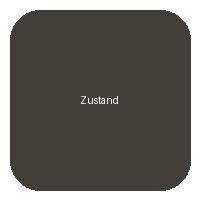
\includegraphics[height=1.4cm]{images/zustand_logo.png}
  \caption{Zustand}
\end{subfigure}
\begin{subfigure}{0.15\textwidth}
  \centering
  
\includegraphics[height=1.4cm]{images/nodejs_logo.png}
  \caption{Node.js 20}
\end{subfigure}
\caption{เทคโนโลยีและเฟรมเวิร์กสำหรับฝั่ง Frontend \& Client}
\end{figure}

\begin{figure}[H]
\centering
\begin{subfigure}{0.18\textwidth}
  \centering
  
\includegraphics[height=1.3cm]{images/aws_logo.png}
  \caption{AWS Cloud}
\end{subfigure}
\begin{subfigure}{0.18\textwidth}
  \centering
  
\includegraphics[height=1.3cm]{images/aws_lambda.png}
  \caption{AWS Lambda}
\end{subfigure}
\begin{subfigure}{0.18\textwidth}
  \centering
  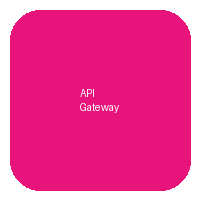
\includegraphics[height=1.3cm]{images/aws_apigateway.png}
  \caption{API Gateway}
\end{subfigure}
\begin{subfigure}{0.18\textwidth}
  \centering
  
\includegraphics[height=1.3cm]{images/aws_dynamodb.png}
  \caption{DynamoDB}
\end{subfigure}
\begin{subfigure}{0.18\textwidth}
  \centering
  
\includegraphics[height=1.3cm]{images/aws_cloudwatch.png}
  \caption{CloudWatch}
\end{subfigure}
\caption{บริการคลาวด์บนสถาปัตยกรรม AWS Serverless}
\end{figure}

\newpage

% ==================== บทที่ 3 ====================
\section{การวิเคราะห์และออกแบบระบบ (System Analysis \& Design)}

\subsection{ข้อกำหนดความต้องการของระบบ (Requirements)}
\begin{itemize}[leftmargin=1.5em, itemsep=2pt]
  \item \textbf{Functional Requirements (FR):}
  \begin{enumerate}[leftmargin=1.5em, itemsep=1pt]
    \item ผู้ใช้สามารถสมัครสมาชิก เข้าสู่ระบบ และถือครอง JWT Token เพื่อยืนยันตัวตนได้
    \item ผู้ใช้สามารถสร้าง แก้ไข คัดลอก และลบเด็คการ์ดส่วนตัวได้
    \item ผู้ใช้สามารถเปิดซองการ์ดสุ่ม (Booster Pack) 12 ใบตามเรตความหายากทางการได้
    \item ผู้ใช้สามารถตรวจสอบการ์ดแบบ 3 มิติ (3D Card Inspector) ดูเอฟเฟกต์ฟอยล์และรายละเอียดการ์ดได้
    \item ผู้ใช้สามารถสร้างหรือเข้าร่วมห้องเล่นการ์ดด้วยรหัสห้อง 6 หลักได้
    \item ผู้ใช้สามารถลากการ์ดลงสนาม หมุนการ์ดคว่ำ/หงาย เพิ่มลด Lore และส่งผลให้ฝ่ายตรงข้ามเห็นแบบเรียลไทม์ได้
    \item ระบบสามารถวิเคราะห์สถิติเด็คการ์ด เช่น ค่าร่ายเฉลี่ย (Ink Curve) และสัดส่วนการ์ดได้
  \end{enumerate}
  \item \textbf{Non-Functional Requirements (NFR):}
  \begin{enumerate}[leftmargin=1.5em, itemsep=1pt]
    \item \textbf{Latency:} ความหน่วงในการซิงค์ข้อมูลผ่าน WebSocket ต้องต่ำกว่า 100 มิลลิวินาที ($<$100ms)
    \item \textbf{Cost:} สถาปัตยกรรมต้องทำงานได้ภายใต้งบประมาณ \$0.00 (AWS Free Tier)
    \item \textbf{Availability \& Scalability:} ขยายขนาดรองรับผู้ใช้งานได้อัตโนมัติโดยไม่มี Downtime
    \item \textbf{Security:} รหัสผ่านต้องได้รับการแฮชด้วย bcrypt (Salt Rounds = 10) และส่งข้อมูลผ่าน HTTPS/WSS
  \end{enumerate}
\end{itemize}

\subsection{การออกแบบสถาปัตยกรรมคลาวด์บน AWS (100\% Serverless)}
ระบบทำงานบนสถาปัตยกรรม Event-Driven Serverless แบ่งเป็น 3 เลเยอร์หลัก:
\begin{enumerate}[leftmargin=1.5em, itemsep=2pt]
  \item \textbf{Presentation Layer:} เว็บแอปพลิเคชัน Single Page Application (SPA) ให้บริการผ่าน HTTPS
  \item \textbf{API \& Routing Layer:} 
  \begin{itemize}[leftmargin=1.5em, itemsep=1pt]
    \item \textbf{HTTP API Gateway:} สำหรับ REST Endpoints (\texttt{/auth/login}, \texttt{/auth/register}, \texttt{/decks})
    \item \textbf{WebSocket API Gateway:} สำหรับการเชื่อมต่อแบบ Persistent Bidirectional Connection (\texttt{\$connect}, \texttt{\$disconnect}, \texttt{\$default})
  \end{itemize}
  \item \textbf{Compute \& Storage Layer:}
  \begin{itemize}[leftmargin=1.5em, itemsep=1pt]
    \item \textbf{AWS Lambda Microservices:} ฟังก์ชันอิสระสำหรับการจัดการสิทธิ์ ข้อมูลเด็ค และห้องเล่น
    \item \textbf{Amazon DynamoDB:} ฐานข้อมูล NoSQL แบบ Document Store ที่มีความหน่วงระดับ Single-digit Millisecond
  \end{itemize}
\end{enumerate}

\subsection{การออกแบบฐานข้อมูลแบบ NoSQL (Amazon DynamoDB Schema)}

\begin{table}[H]
\centering
\small
\begin{tabular}{p{3cm} p{2.2cm} p{2.2cm} p{3.8cm} p{3.2cm}}
\toprule
\textbf{ตาราง} & \textbf{Partition Key} & \textbf{Sort Key} & \textbf{Attributes สำคัญ} & \textbf{วัตถุประสงค์} \\
\midrule
\texttt{LorcanaUsers} & \texttt{userId} (S) & - & \texttt{username}, \texttt{passwordHash}, \texttt{createdAt} & เก็บข้อมูลผู้ใช้และแฮชรหัสผ่าน \\
\texttt{LorcanaDecks} & \texttt{userId} (S) & \texttt{deckId} (S) & \texttt{deckName}, \texttt{inks}, \texttt{cards} (List), \texttt{updatedAt} & เก็บรายการเด็คการ์ดของผู้ใช้ \\
\texttt{LorcanaRoomState} & \texttt{roomId} (S) & \texttt{connectionId} (S) & \texttt{username}, \texttt{role}, \texttt{state} (JSON), \texttt{ttl} & เก็บสถานะห้องและ WebSocket \\
\bottomrule
\end{tabular}
\caption{โครงสร้างตารางฐานข้อมูล Amazon DynamoDB}
\end{table}

\subsection{ลำดับขั้นตอนการสื่อสารแบบเรียลไทม์ (WebSocket Sequence Flow)}
\begin{enumerate}[leftmargin=1.5em, itemsep=2pt]
  \item \textbf{การสร้าง/เข้าร่วมห้อง (\texttt{JOIN\_ROOM}):} ผู้เล่นส่งคำขอ \texttt{JOIN\_ROOM} พร้อมรหัสห้อง 6 หลัก API Gateway เรียก Lambda Room Router เพื่อลงทะเบียน Connection ID ลงใน \texttt{LorcanaRoomState}
  \item \textbf{การอัปเดตสถานะกระดาน (\texttt{CARD\_MOVED} / \texttt{CARD\_EXERTED}):} เมื่อผู้เล่นลากการ์ดหรือเปลี่ยนสถานะ Client จะทำการ Optimistic Update ที่หน้าจอทันที และส่ง Action Payload ไปยัง WebSocket API Gateway
  \item \textbf{การส่งต่อข้อมูล (Relay \& Broadcast):} Lambda Room Router อ่าน Connection ID ของฝ่ายตรงข้ามจาก DynamoDB และใช้ \texttt{@connections} API เพื่อ Broadcast ข้อความไปยังคู่แข่งภายในเวลา $<$100ms
\end{enumerate}

\subsection{กฎกติกาและองค์ประกอบของเกมการ์ด Disney Lorcana}

\begin{figure}[H]
\centering
\begin{subfigure}{0.15\textwidth}
  \centering
  
\includegraphics[height=1.5cm]{images/Amber.png}
  \caption{Amber}
\end{subfigure}
\begin{subfigure}{0.15\textwidth}
  \centering
  
\includegraphics[height=1.5cm]{images/Amethyst.png}
  \caption{Amethyst}
\end{subfigure}
\begin{subfigure}{0.15\textwidth}
  \centering
  
\includegraphics[height=1.5cm]{images/Emerald.png}
  \caption{Emerald}
\end{subfigure}
\begin{subfigure}{0.15\textwidth}
  \centering
  
\includegraphics[height=1.5cm]{images/ruby.png}
  \caption{Ruby}
\end{subfigure}
\begin{subfigure}{0.15\textwidth}
  \centering
  
\includegraphics[height=1.5cm]{images/sapphire.png}
  \caption{Sapphire}
\end{subfigure}
\begin{subfigure}{0.15\textwidth}
  \centering
  
\includegraphics[height=1.5cm]{images/steel.png}
  \caption{Steel}
\end{subfigure}
\caption{หมวดหมู่สีหมึกทั้ง 6 สีของเกม Disney Lorcana}
\end{figure}

ระบบจำลององค์ประกอบหลักของเกมตามกติกาทางการ:
\begin{itemize}[leftmargin=1.5em, itemsep=2pt]
  \item \textbf{6 หมวดสีหมึก (Ink Types):} Amber (สนับสนุน), Amethyst (เวทมนตร์), Emerald (ความยืดหยุ่น), Ruby (โจมตีรวดเร็ว), Sapphire (ทรัพยากร/ปัญญา), Steel (พลังป้องกัน)
  \item \textbf{ประเภทการ์ด (Card Types):} Character, Action/Song, Item, Location
  \item \textbf{สถานะการ์ด (Card States):} Ready (แนวตั้ง พร้อมใช้งาน) และ Exerted (แนวนอน พักการใช้งาน)
  \item \textbf{เป้าหมายของเกม:} ผู้เล่นที่สะสมแต้มความรู้ (Lore) ครบ 20 แต้มก่อนจะเป็นผู้ชนะ
\end{itemize}

\newpage

% ==================== บทที่ 4 ====================
\section{การพัฒนาระบบและผลการดำเนินงาน (Implementation \& Test Results)}

\subsection{การพัฒนาส่วนติดต่อผู้ใช้ (Frontend Implementation \& Playmat UI)}
ส่วนติดต่อผู้ใช้ได้รับการออกแบบตามแนวคิด \textbf{Dark Editorial + Magic R3} เพื่อมอบประสบการณ์ระดับพรีเมียม:

\begin{figure}[H]
\centering
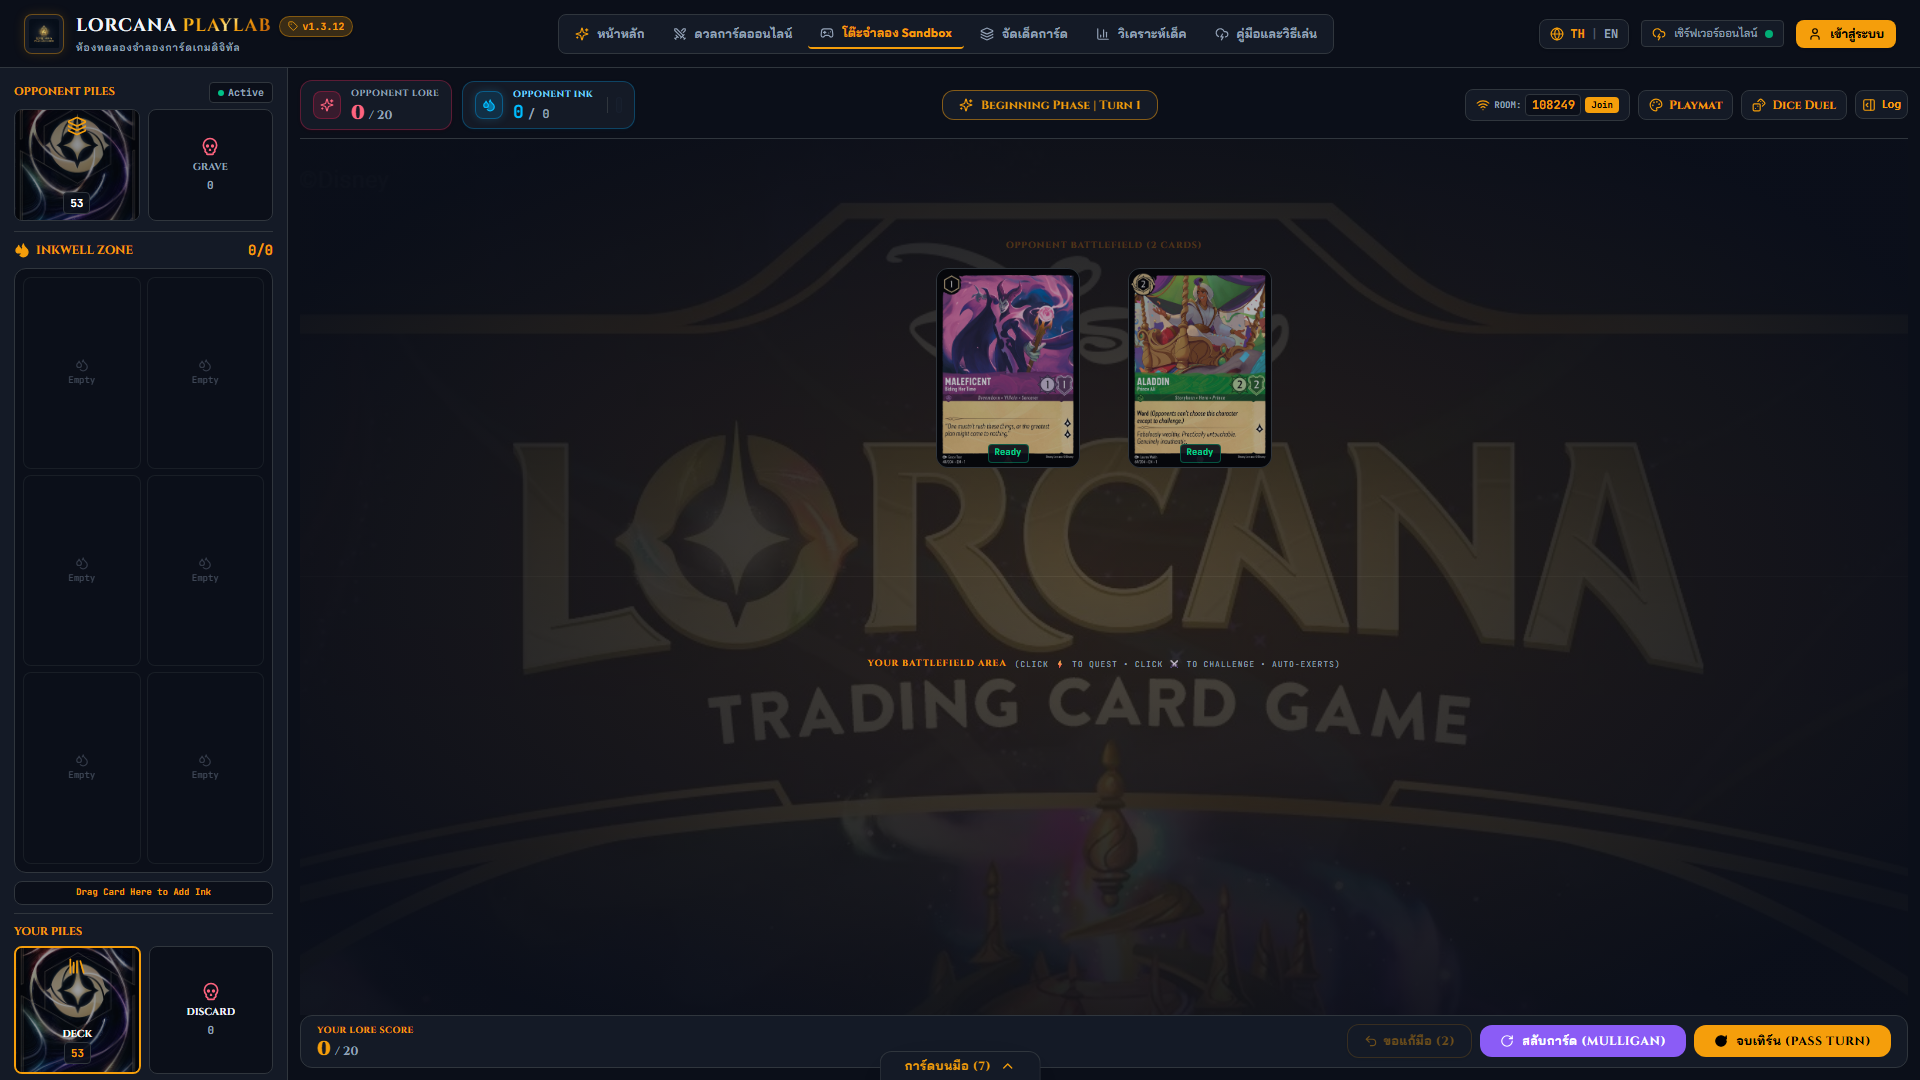
\includegraphics[width=0.88\textwidth]{images/screenshot_board_playing.png}
\caption{หน้าจอกระดานจำลองการเล่นการ์ด (Lorcana Board Simulation) พร้อมระบบลากวางและ 3D Physics}
\end{figure}

\begin{figure}[H]
\centering
\begin{subfigure}{0.48\textwidth}
  \centering
  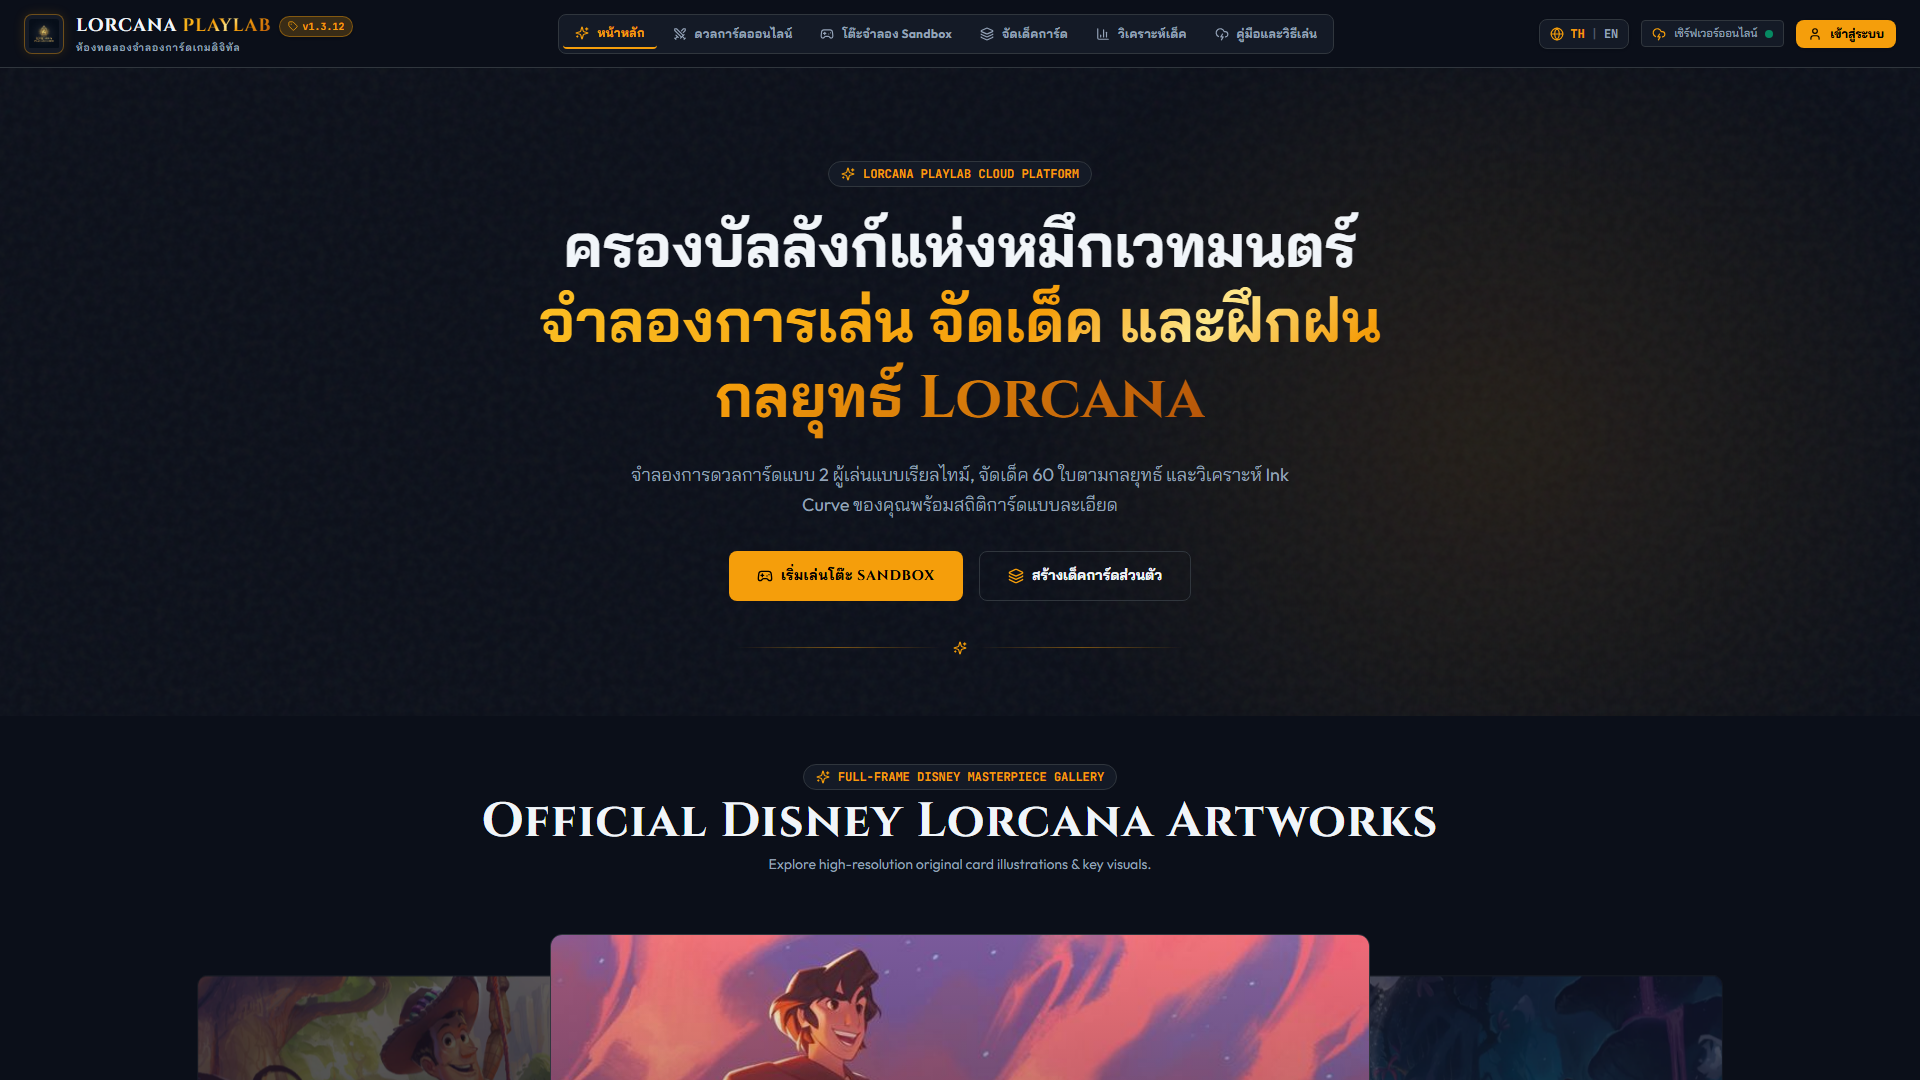
\includegraphics[width=\textwidth]{images/screenshot_hub.png}
  \caption{Game Hub แดชบอร์ดหลัก}
\end{subfigure}
\hfill
\begin{subfigure}{0.48\textwidth}
  \centering
  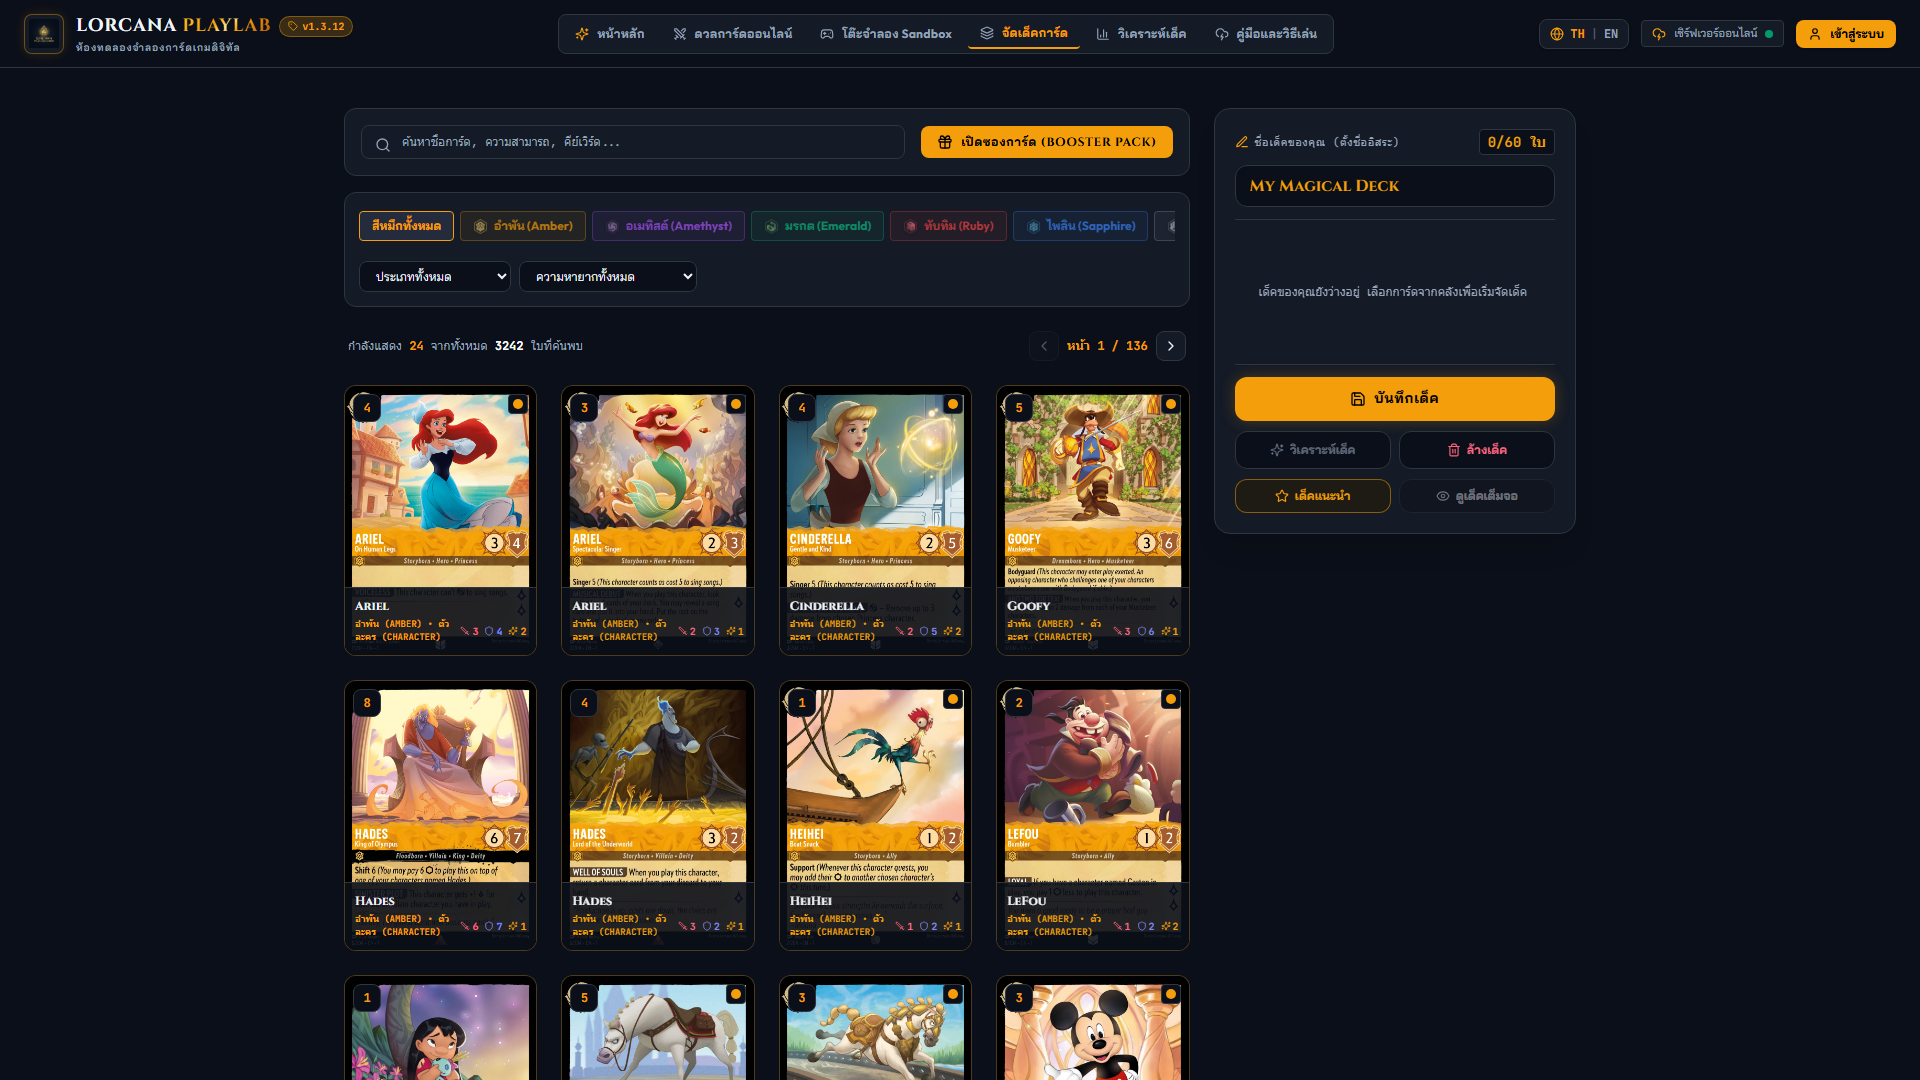
\includegraphics[width=\textwidth]{images/screenshot_deckbuilder.png}
  \caption{ระบบจัดเด็คการ์ด (Deck Builder)}
\end{subfigure}
\\[6pt]
\begin{subfigure}{0.48\textwidth}
  \centering
  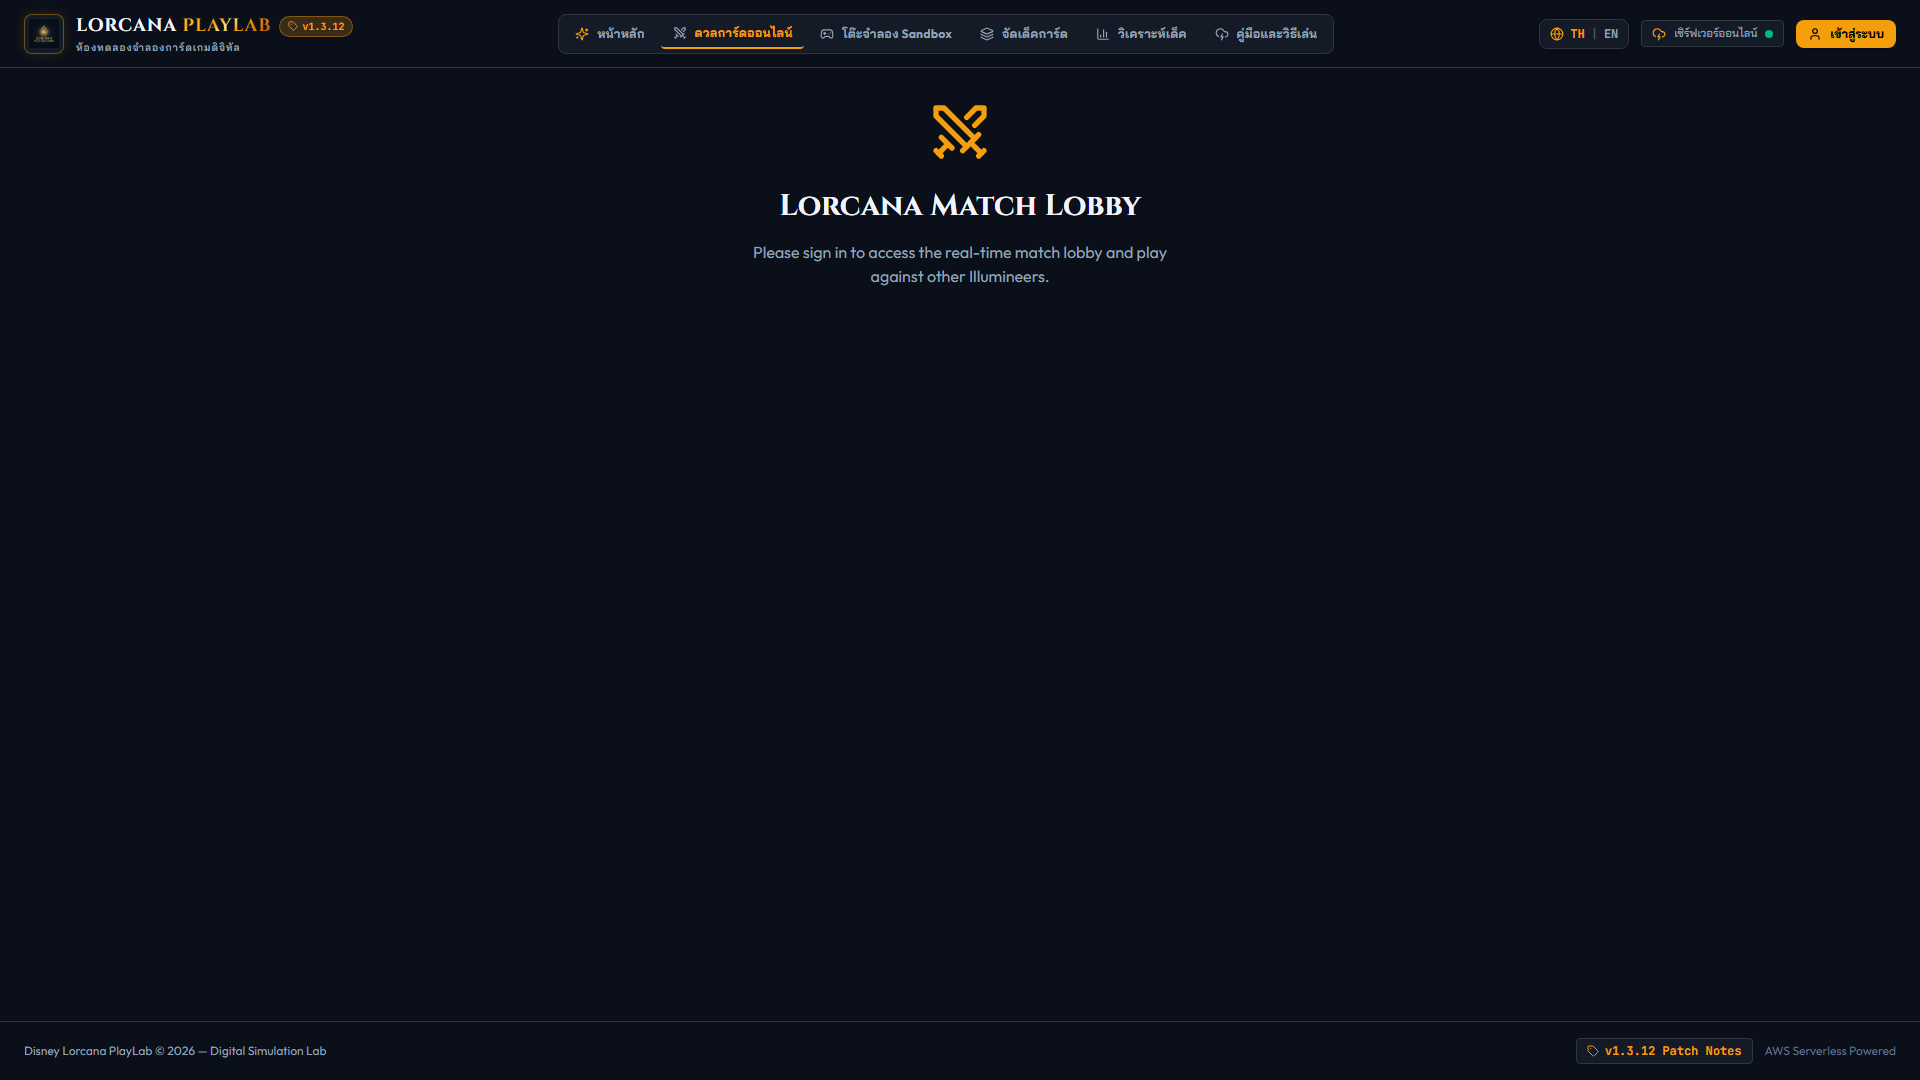
\includegraphics[width=\textwidth]{images/screenshot_matchlobby.png}
  \caption{ระบบห้องเล่นเรียลไทม์ (Match Lobby)}
\end{subfigure}
\hfill
\begin{subfigure}{0.48\textwidth}
  \centering
  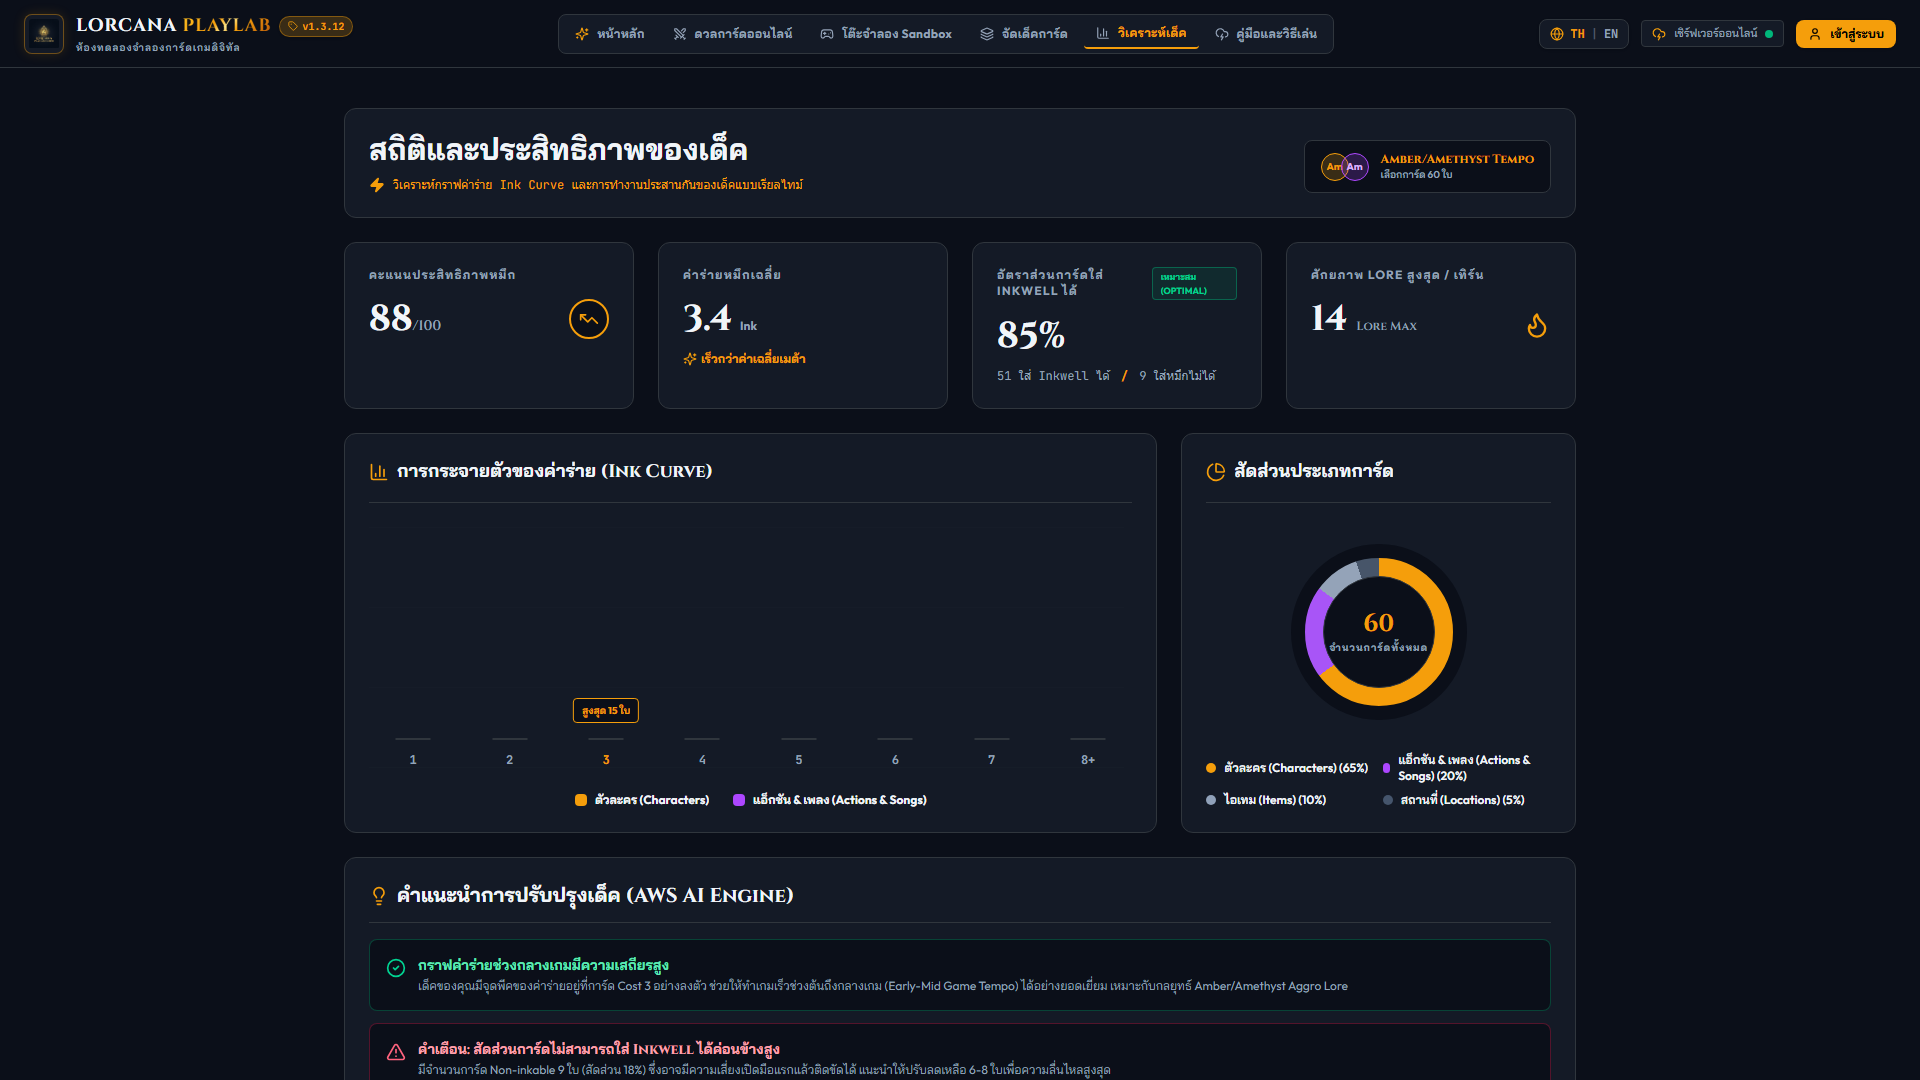
\includegraphics[width=\textwidth]{images/screenshot_analytics.png}
  \caption{ระบบวิเคราะห์เด็ค (Deck Analytics)}
\end{subfigure}
\caption{ภาพหน้าจอส่วนติดต่อผู้ใช้หลักของระบบ Disney Lorcana PlayLab Cloud}
\end{figure}

\begin{figure}[H]
\centering
\begin{subfigure}{0.48\textwidth}
  \centering
  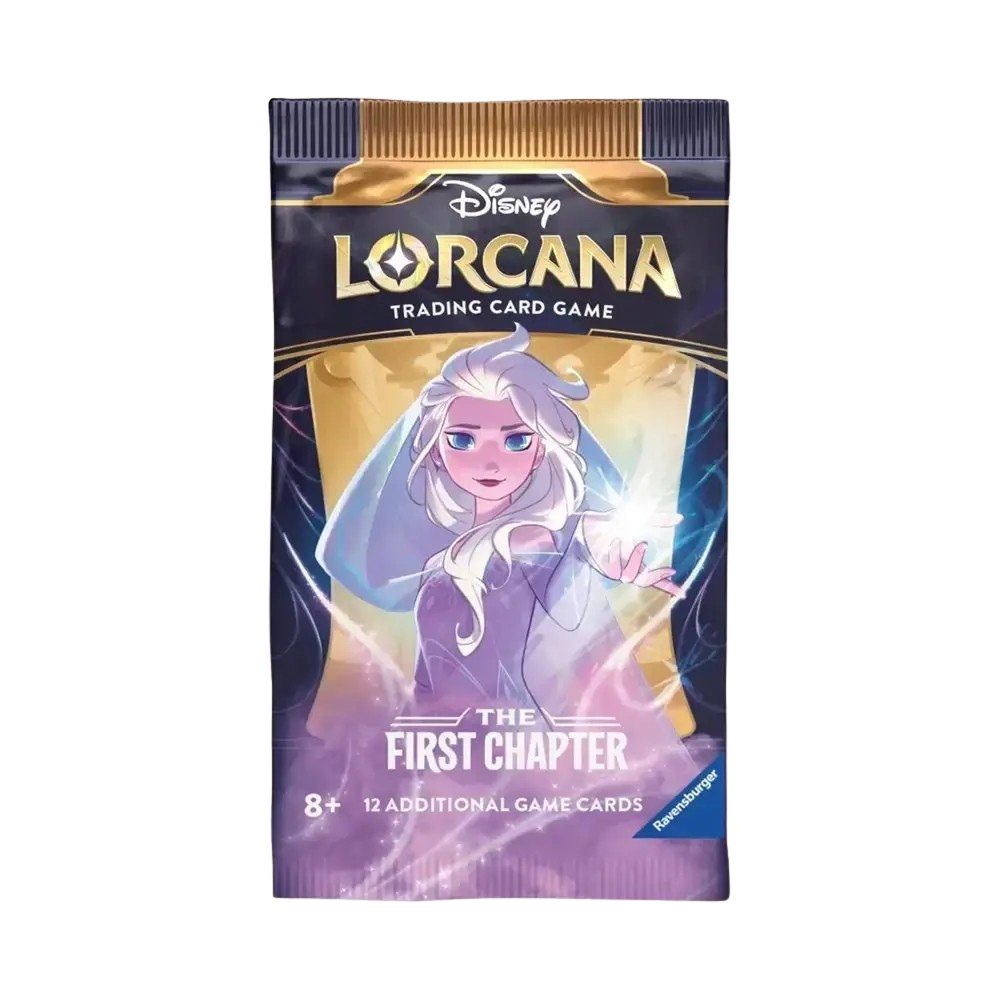
\includegraphics[width=\textwidth]{images/CardGachaDisney.png}
  \caption{แอนิเมชันเปิดซองการ์ดสุ่ม (Booster Pack)}
\end{subfigure}
\hfill
\begin{subfigure}{0.48\textwidth}
  \centering
  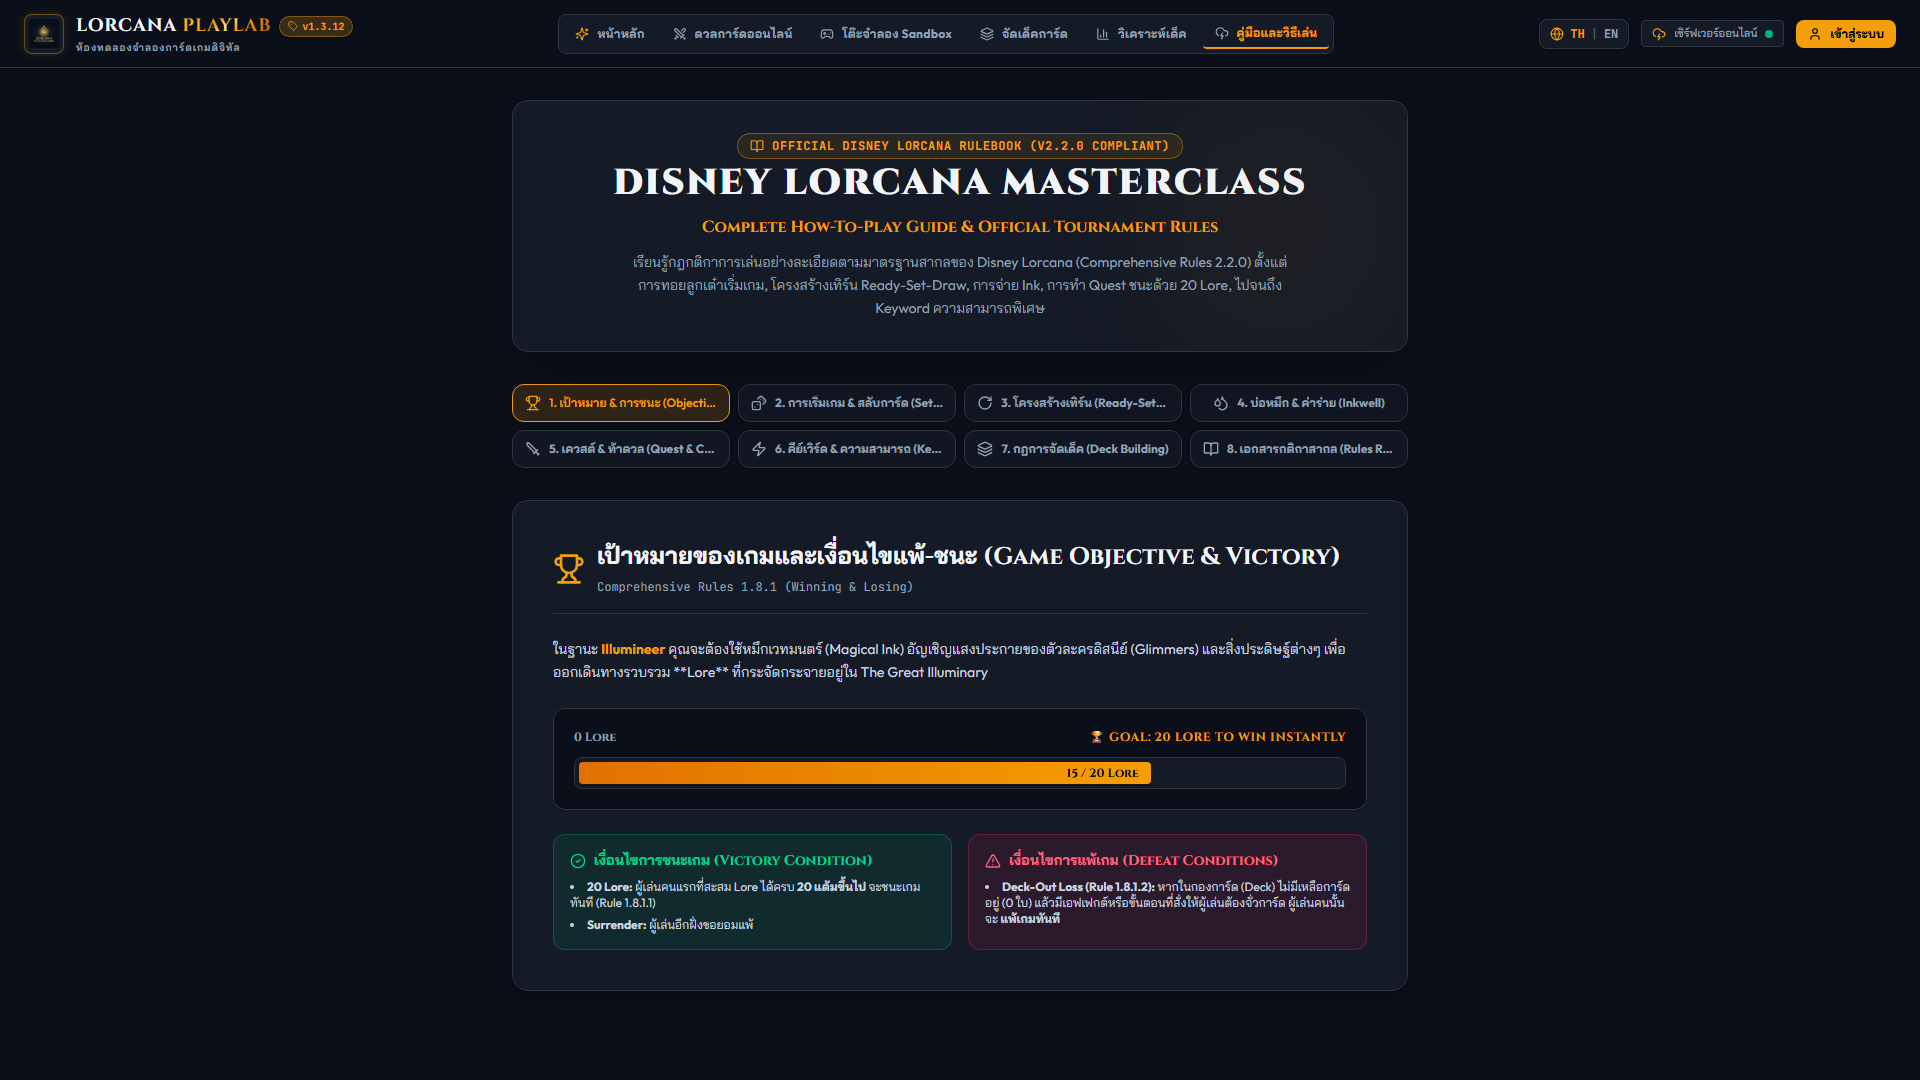
\includegraphics[width=\textwidth]{images/screenshot_rules.png}
  \caption{คู่มือกฎกติกาและการเล่น (Rules \& Guide)}
\end{subfigure}
\caption{ระบบเปิดซองการ์ดสุ่มและคู่มือการเล่น}
\end{figure}

\subsection{การพัฒนาส่วนประมวลผลบนคลาวด์ (AWS Backend Microservices)}
ฟังก์ชัน Lambda ได้รับการพัฒนาด้วย TypeScript และคอมไพล์เป็น Node.js 20.x:
\begin{itemize}[leftmargin=1.5em, itemsep=2pt]
  \item \textbf{\texttt{lorcana-auth-register} \& \texttt{lorcana-auth-login}:} ตรวจสอบข้อมูล เข้ารหัสผ่านด้วย bcrypt และออก JWT Token
  \item \textbf{\texttt{lorcana-deck}:} จัดการ CRUD เด็คการ์ด โดยแยก Route ตาม HTTP Method (GET, POST, PUT, DELETE)
  \item \textbf{\texttt{lorcana-room-handler}:} จัดการการเชื่อมต่อ WebSocket, ถอดรหัส Action, บันทึก Session ลง DynamoDB และ Broadcast ข้อมูลผ่าน ApiGatewayManagementApi
\end{itemize}

\subsection{การแก้ปัญหาข้อจำกัดบน AWS Learner Lab}
ในการปรับใช้ระบบจริงบน AWS Learner Lab ทีมงานพบข้อจำกัดด้านความปลอดภัยที่บล็อกคำสั่ง \texttt{iam:CreateRole} ส่งผลให้ไม่สามารถรันคำสั่ง \texttt{sam deploy} แบบอัตโนมัติได้ ทีมงานจึงได้แก้ไขปัญหาอย่างเป็นระบบ:
\begin{enumerate}[leftmargin=1.5em, itemsep=2pt]
  \item \textbf{การใช้ LabRole สำเร็จรูป:} ปรับใช้ \texttt{LabRole} ที่ระบบจัดเตรียมไว้ให้แทนการสร้าง IAM Role ใหม่
  \item \textbf{สคริปต์ Manual Deployment (\texttt{scripts/deploy\_manual.sh}):} พัฒนาสคริปต์คอมไพล์โค้ด สร้างไฟล์ ZIP และอัปเดตโค้ดขึ้น Lambda โดยตรงผ่าน AWS CLI
  \item \textbf{การแก้ไข API Gateway Payload Format Version:} เปลี่ยน Integration จาก v2.0 เป็น v1.0 เพื่อให้ตรงกับ \texttt{APIGatewayProxyEvent} ของ Lambda
  \item \textbf{การจัดทำ Route Integration Mapping:} ตรวจสอบและแก้ไข Integration URI ให้ชี้ไปยัง Lambda Function ที่ถูกต้องอย่างแม่นยำ
\end{enumerate}

\subsection{ผลการทดสอบระบบแบบ End-to-End (End-to-End Testing)}

\begin{table}[H]
\centering
\small
\begin{tabular}{p{3.2cm} p{4cm} p{3.2cm} p{3cm} p{1.2cm}}
\toprule
\textbf{Endpoint / Action} & \textbf{Test Case / Payload} & \textbf{ผลลัพธ์ที่คาดหวัง} & \textbf{ผลการทดสอบจริง} & \textbf{สถานะ} \\
\midrule
\texttt{POST /auth/register} & \texttt{\{"username":"tawan",...\}} & HTTP 201 Created & 201 User registered & \textbf{ผ่าน} \\
\texttt{POST /auth/login} & \texttt{\{"username":"tawan",...\}} & HTTP 200 + JWT Token & 200 Login + Token & \textbf{ผ่าน} \\
\texttt{POST /decks} & \texttt{\{"deckName":"Ruby Control"\}} & HTTP 201 บันทึก DynamoDB & 201 Deck saved & \textbf{ผ่าน} \\
\texttt{GET /decks} & \texttt{Bearer <token>} & HTTP 200 คืนรายการเด็ค & 200 คืนรายการครบถ้วน & \textbf{ผ่าน} \\
\texttt{DELETE /decks/\{id\}} & Path Parameter \texttt{deckId} & HTTP 200 ลบเด็คสำเร็จ & 200 Deck deleted & \textbf{ผ่าน} \\
\texttt{WSS \$connect} & \texttt{wss://a86238wqo4.../prod} & HTTP 101 Switching & เชื่อมต่อ Socket สำเร็จ & \textbf{ผ่าน} \\
\texttt{WSS JOIN\_ROOM} & \texttt{\{"action":"JOIN\_ROOM",...\}} & บันทึก DynamoDB & 200 เข้าร่วมห้องสำเร็จ & \textbf{ผ่าน} \\
\texttt{WSS CARD\_MOVED} & \texttt{\{"action":"CARD\_MOVED",...\}} & Relay ไปยังคู่แข่ง & ส่งถึงคู่แข่งใน $<$100ms & \textbf{ผ่าน} \\
\bottomrule
\end{tabular}
\caption{ตารางสรุปผลการทดสอบระบบแบบ End-to-End บนสภาพแวดล้อม AWS Production}
\end{table}

\newpage

% ==================== บทที่ 5 ====================
\section{การประเมินค่าใช้จ่ายบนคลาวด์และแผนงานขั้นต่อไป (Cost Assessment \& Future Roadmap)}

\subsection{การประเมินค่าใช้จ่ายสถาปัตยกรรมคลาวด์ (AWS Free Tier Optimization)}
จากการคำนวณผ่าน AWS Pricing Calculator สำหรับปริมาณการใช้งานระดับ 10,000 ผู้เล่นต่อเดือน:
\begin{itemize}[leftmargin=1.5em, itemsep=2pt]
  \item \textbf{AWS Lambda:} 1,000,000 Requests ฟรีต่อเดือน (การใช้งานจริงประมาณ 250,000 Requests = \$0.00)
  \item \textbf{Amazon DynamoDB:} ฟรี 25 GB Storage และ 25 WCU / 25 RCU (การใช้งานจริง $<$ 1 GB = \$0.00)
  \item \textbf{AWS API Gateway (HTTP \& WebSocket):} 1,000,000 Messages ฟรีใน Free Tier (\$0.00)
  \item \textbf{Amazon SQS:} 1,000,000 Requests ฟรีต่อเดือน (\$0.00)
  \item \textbf{Amazon CloudWatch:} 5 GB Log Data Ingestion ฟรีต่อเดือน (\$0.00)
\end{itemize}

\textbf{สรุปค่าใช้จ่ายรวมทั้งสิ้น:} \textbf{\$0.00 ต่อเดือน} สอดคล้องกับเป้าหมายการควบคุมงบประมาณของโครงงาน

\subsection{แผนงานพัฒนาสำหรับ Sprint 4 และ Sprint 5}
\begin{enumerate}[leftmargin=1.5em, itemsep=2pt]
  \item \textbf{Sprint 4 (Deck Analyzer Microservice):} พัฒนาระบบประมวลผลวิเคราะห์สมดุลเด็คแบบ Asynchronous โดยใช้ Amazon SQS รับงานและทริกเกอร์ Lambda ในการคำนวณความเสี่ยง ค่าร่าย และความเข้ากันได้ของการ์ด
  \item \textbf{Sprint 5 (Observability \& Security Hardening):} ย้ายค่าความลับ (JWT Secret) ไปจัดเก็บใน AWS Secrets Manager และตั้งค่า CloudWatch Dashboard พร้อมระบบแจ้งเตือน Error Rate เกิน 1\%
  \item \textbf{Sprint 6 (Load Testing \& Resilience):} ทดสอบประสิทธิภาพระบบด้วยเครื่องมือ Artillery ภายใต้โหลด 500 Concurrent Connections พร้อมระบบเชื่อมต่อใหม่อัตโนมัติ (WebSocket Auto-reconnect) เมื่อสัญญาณหลุด
\end{enumerate}

\subsection{สรุปผลการดำเนินงานและบทเรียนที่ได้รับ (Sprint Retrospective)}
การพัฒนาโครงงาน Disney Lorcana PlayLab Cloud ใน Sprint 1 ถึง 3 บรรลุเป้าหมายตามเกณฑ์การประเมิน Stage 2 อย่างครบถ้วน บทเรียนสำคัญที่ได้รับจากการปฏิบัติงานจริง ได้แก่:
\begin{enumerate}[leftmargin=1.5em, itemsep=2pt]
  \item \textbf{ความสำคัญของ Spec และ Interface Design:} การกำหนด Schema ของ WebSocket Payload และ DynamoDB อย่างรอบคอบช่วยให้การทำงานร่วมกันระหว่าง Frontend และ Backend ราบรื่น
  \item \textbf{การทำความเข้าใจข้อจำกัดของสภาพแวดล้อมคลาวด์:} การปรับใช้สคริปต์ Manual Deployment ช่วยให้ทีมสามารถเอาชนะข้อจำกัดสิทธิ์บน AWS Learner Lab ได้อย่างมีประสิทธิภาพ
  \item \textbf{การตรวจสอบ Integration Mapping:} การจับคู่วิธีการส่งถ่ายข้อมูลระหว่าง API Gateway และ Lambda ต้องสอดคล้องกับเวอร์ชันของ Payload Format เพื่อป้องกันข้อผิดพลาด 405 Method Not Allowed
\end{enumerate}

\newpage

% ==================== เอกสารอ้างอิง ====================
\begin{thebibliography}{99}
\addcontentsline{toc}{section}{เอกสารอ้างอิง (References)}

\bibitem{lorcana}
Ravensburger \& Disney. (2023). \textit{Disney Lorcana Trading Card Game Official Rules and Card Database}. \url{https://www.disneylorcana.com}

\bibitem{awslambda}
Amazon Web Services. (2026). \textit{Building Event-Driven Architectures with AWS Lambda and Amazon DynamoDB}. AWS Documentation. \url{https://docs.aws.amazon.com/lambda/}

\bibitem{awswebsocket}
Amazon Web Services. (2026). \textit{About WebSocket APIs in API Gateway}. AWS Documentation. \url{https://docs.aws.amazon.com/apigateway/latest/developerguide/apigateway-websocket-api.html}

\bibitem{react19}
React Working Group. (2026). \textit{React 19 Documentation and Concurrent Features}. \url{https://react.dev}

\bibitem{tailwind}
Tailwind Labs. (2026). \textit{Tailwind CSS v4.0 Alpha/Release Documentation}. \url{https://tailwindcss.com}

\bibitem{framer}
Framer. (2026). \textit{Framer Motion: Production-ready animation library for React}. \url{https://www.framer.com/motion/}

\end{thebibliography}

\end{document}
